\section{Introduction}

%\xxx{Old Story: building on Merkle etc we build cryptography out of combinatorial assumptions. We get a fine-grained key exchange from fine-grained assumptions, instead of from assumptions of an exponential gap! We demonstrate other changes needed to get one way functions with desired properties. We give the general form of what is needed to build the desired objects. Our assumptions seem like "One way function" type assumptions and combinatorial ones, and yet we can build a key exchange. }

% Abstract


Modern cryptography has developed a variety of important cryptographic primitives, from One-Way Functions (OWFs) to Public-Key Cryptography to Obfuscation. 
Except for a few more limited information theoretic results \cite{Shamir79,CKGS98,RW02}, cryptography has so far required making a computational assumption, P $\neq$ NP being a baseline requirement.
Barring unprecedented progress in computational complexity, such hardness hypotheses seem necessary in order to obtain most useful primitives. 
To alleviate this reliance on unproven assumptions, it is good to build cryptography from a variety of extremely different, believable assumptions: if a technique disproves one hypothesis, the unrelated ones might still hold. Due to this, there are many different cryptographic assumptions: on factoring, discrete logarithm, shortest vector in lattices and many more.

%** - Discrete logarithm is an optioon

% (Secret-sharing, PIR, entropic security, quantum??)


Unfortunately, almost all hardness assumptions used so far have the same quite stringent requirements: not only that NP is not in BPP, but that we must be able to efficiently sample polynomially-hard instances whose solution we know. Impagliazzo \cite{Impagliazzo5worlds,RR94} defined five worlds, which capture the state of cryptography, depending on which assumptions happen to fail. The three worlds worst for cryptography are Algorithmica (NP in BPP), Heuristica (NP is not in BPP but NP problems are easy on average) and Pessiland (there are NP problems that are hard on average but solved hard instances are hard to sample, and OWFs do not exist). 
This brings us to our main question.

\begin{center}
 \emph{	Can we have a meaningful notion of cryptography even if we live in Pessiland (or Algorithmica or Heuristica)?}
\end{center}

This question motivates a weaker notion of cryptography: cryptography that is secure against $n^k$-time bounded adversaries, for a constant $k$. Let us see why such cryptography might exist even if P $=$ NP. In complexity, for most interesting computational models, we have time hierarchy theorems that say that there are problems solvable in $O(n^2)$ time (say) that cannot be solved in $O(n^{2-\epsilon})$ time for any $\epsilon>0$ \cite{HS65,HS66,Tse56}. In fact, such theorems exist also for the average case time complexity of problems \cite{Lev73}. Thus, even if P$=$NP, there are problems that are hard on average for specific runtimes, i.e. {\em fine-grained} hard on average. {\em Can we use such hard problems to build useful cryptographic primitives?} 

Unfortunately, the problems from the time hierarchy theorems are difficult to work with, a common problem in the search for unconditional results. Thus, let us relax our requirements and consider hardness assumptions, but this time on the exact running time of our problems of interest. One simple approach is to consider all known constructions of Public Key Cryptography (PKC) to date and see what they imply if the hardness of the underlying problem is relaxed to be $n^{k-o(1)}$ for a fixed $k$ (as it would be in Pessiland). Some of the known schemes are extremely efficient. For instance, the RSA and Diffie-Hellman cryptosystems immediately imply weak PKC if one changes their assumptions to be about polynomial hardness \cite{rsa,DiffieHellman}. However, these cryptosystems have other weaknesses -- for instance, they are completely broken in a postquantum world as Shor's algorithm breaks their assumptions in essentially quadratic time \cite{Shor}. Thus, it makes sense to look at the cryptosystems based on other assumptions. Unfortunately, largely because cryptography has mostly focused on the gap between polynomial and superpolynomial time, most reductions building PKC have a significant (though polynomial) overhead; many require, for example, multiple rounds of Gaussian elimination. As a simple example,
the Goldreich-Levin  construction for hard-core bits uses $n^{\omega}$ (where $\omega\in [2,2.373)$ is the exponent of square matrix multiplication \cite{VVWmmfaster}\cite{legallMM}) time and $n$ calls to the hard-core-bit distinguisher \cite{hardCoreBitsAndXorLemmaFromGL}. The polynomial overhead of such reductions means that if the relevant problem is only $n^{2-o(1)}$ hard, instead of super-polynomially hard, the reduction will not work anymore and won't produce a meaningful cryptographic primitive. Moreover, reductions with fixed polynomial overheads are no longer composable in the same way when we consider weaker, polynomial gap cryptography. Thus, new, more careful cryptographic reductions are needed.

Ball et al.~\cite{avgCaseFineGrained,eprintAvgCaseFG} recently began to address this issue through the lens of the recently blossoming field of {\em fine-grained complexity}.
%The main idea is as follows:
%While the problems from the time hierarchy theorems seem difficult to work with, there are several very simple, structured problems that are conjectured to require $n^{2-o(1)}$ time to solve on average, say on a RAM. These problems come from a recently blossoming field: fine-grained complexity, 
Fine-grained complexity is built upon ``fine-grained'' hypotheses on the (worst-case) hardness of a small number of key problems. Each of these key problems $K$, has a simple algorithm using a combination of textbook techniques, running in time $T(n)$ on instances of size $n$, in, say, the RAM model of computation. However, despite decades of research, no $\~O(T(n)^{1-\epsilon})$ algorithm is known for any $\epsilon>0$ (note that the tilde $~$ suppresses sub-polynomial factors). The fine-grained hypothesis for $K$ is then that $K$ requires $T(n)^{1-o(1)}$ time in the RAM model of computation. Some of the main hypotheses in fine-grained complexity (see \cite{icm-survey}) set $K$ to be CNF-SAT (with $T(n)=2^n$, where $n$ is the number of variables), or the \kSum~problem (with $T(n)=n^{\lceil k/2\rceil}$), or the All-Pairs Shortest Paths problem (with $T(n)=n^3$ where $n$ is the number of vertices), or one of several versions of the $k$-Clique problem in weighted graphs.
Fine-grained uses fine-grained reductions between problems in a very tight way (see \cite{icm-survey}): if problem $A$ has requires running time $a(n)^{1-o(1)}$, and one obtains an $(a(n),b(n))$-fine-grained reduction from $A$ to $B$, then problem $B$ needs runtime $b(n)^{1-o(1)}$. Using such reductions, one can obtain strong lower bounds for many problems, conditioned on one of the few key hypotheses.


%While fine-grained complexity is typically about worst-case hardness assumptions, several of its key hard problems are conjectured to also be hard on average: e.g. $k$-SUM where the range of the integers is roughly between $-n^k$ and $n^k$. 

The main question that Ball et al. set out to answer is: {\em Can one use fine-grained reductions from the hard problems from fine-grained complexity to build useful cryptographic primitives?} Their work produced worst-case to average-case fine-grained reductions from key problems to new algebraic average case problems. %to a new problem %that can be solved in roughly the same time for each of several key problems from fine-grained complexity. 
%This gave, for example, a problem that requires $n^{2-o(1)}$ time to solve on average, based on the \ThSum~conjecture. 
From these new problems, Ball et al. were able to construct fine-grained proofs of work, but they were not able to obtain stronger cryptographic primitives such as fine-grained one-way-functions or public key encryption. In fact, they gave a barrier for their approach: extending their approach would falsify the Nondeterministic Strong Exponential Time Hypothesis (NSETH) of Carmosino et al. \cite{CarmosinoGIMPS16}. Because of this barrier, one would either need to develop brand new techniques, or use a different hardness assumption.

\begin{center}{\em What kind of hardness assumptions can be used to obtain public-key cryptography (PKC) even in Pessiland?}\end{center} 

A great type of theorem to address this would be: for every problem $P$ that requires $n^{k-o(1)}$ time on average, one can construct a public-key exchange (say), for which Alice and Bob can exchange a $\lg(n)$ bit key in time $O(n^{ak})$, whereas Eve must take $n^{(a+g)k-o(1)}$ time to learn Alice and Bob's key, where $g$ is large, and $a$ is small. As a byproduct of such a theorem, one can obtain not just OWFs, but even PKC in Pessiland under fine-grained assumptions via the results of Ball et al. Of course, due to the limitations given by Ball et al. such an ideal theorem would have to refute NSETH, and hence would be at the very least difficult to prove.
Thus, let us relax our goal, and ask 
%\begin{center}{\em What properties does a fine-grained average-case assumption need to have so that fine-grained PKC can be built from it?}\end{center} 
\begin{center}{\em What properties are sufficient for a fine-grained average-case assumption so that it implies fine-grained PKC?}\end{center} 

If we could at least resolve this question, then we could focus our search for worst-case to average-case reductions in a useful way.



%We consider Exact-Weight 3-Clique, which is a key problem, from fine-grained complexity, and show how to build weak public key encryption from it: here the encryption and decryption can be done in time $O(N)$, whereas an adversary needs at least $N^{1.25 - o(1)}$ time.\footnote{We actually approach $N^{1.5 - o(1)}$ if we make the assumption for exact-$k$-clique for large $k$.} While the guarantees are weak, and conditional, our work is the first to show that some sort of public key cryptography can exist in a world where our typical cryptographic assumptions may not hold. 


%In this paper we design \emph{weak} public-key cryptography from polynomial assumptions, providing the possibility of having cryptography in Algorithmica, Heuristica, and Pessiland based, making average-case assumptions on problems from fine-grained complexity.


%\paragraph{Fine-Grained Complexity.} A recently blossoming field is fine-grained complexity, built upon ``fine-grained'' hypotheses on the hardness of a small number of combinatorial problems. These problems have the following in common: each problem $A$, has a simple, textbook algorithm, running in time $T(n)$ on instances of size $n$, in, say, the word-RAM model of computation with $O(\log n)$ bit words. However, despite decades of research, no $\~O(T(n)^{1-\epsilon})$ algorithm is known for any $\epsilon>0$. The fine-grained hypothesis for $A$ is then that $A$ requires $T(n)^{1-o(1)}$ time in the word-RAM model of computation with $O(\log n)$ bit words. Some of the main hypotheses in fine-grained complexity (see \cite{icm-survey}) set $A$ to be CNF-SAT, or the $k$-SUM problem, or the All-Pairs Shortest Paths problem, or one of several versions of the $k$-Clique problem in weighted graphs.

%Fine-grained complexity is concerned with worst-case time complexity. To build cryptography however, we need hypotheses that are about the average-case. Ball, Rosen, Sabin, and Vasudevan \cite{avgCaseFineGrained}
%showed that one can indeed obtain problems that are hard on average, in a fine-grained sense. They established useful definitions of fine-grained one-way functions, and derived the first proof-of-work in a fine-grained setting, based on a worst-case assumption from fine-grained complexity. However, their approach was not sufficient to give a construction of one-way-functions, and indeed Ball et al. proved a limitation of their approach in this regard - extending their approach would falsify the Nondeterministic Strong Exponential Time Hypothesis of Carmosino et al. \cite{CarmosinoGIMPS16}. Because of this seeming barrier, one would either need to develop brand new techniques, or use a different hardness assumption.


%\paragraph{How powerful are polynomial-time fine-grained assumptions?}
%One may be concerned that a polynomial time fine-grained assumption is as strong as a cryptographic assumption about $2^{n}$-time hardness, or at least as strong as assuming that exponentially-hard OWFs exist. It turns out that the two kinds of assumptions are fundamentally different. In a nutshell, traditional cryptography implies fine-grained variants, but not the other way around, and so the fine-grained variants could survive even if all traditional cryptography is somehow broken. 
%%Moreover, fine-grained hardness assumptions on polynomial-time problems are generally orthogonal to super-polynomial hardness assumptions.
%
%As an example, just consider the difference between a polynomially-strong OWF $f_{poly}$ and a fine-grained OWF $f_{fg}$, which we will define informally now. For inputs of length $n$, $f_{poly}$ can be evaluated in time $p(n)$ for some polynomial in $n$ and the time required to inverted it is $2^{\Omega(n)}$. $f_{fg}$ can also be evaluated in time $p'(n)$ for some polynomial in $n$, but the time required to inverted it is merely $p'(n)^{1 + \ell-o(1)}$ for some constant $\ell > 0$. Notice that $f_{poly}$ is already a fine-grained OWF. In this sense, the fine-grained version is strictly weaker, and such fine-grained OWF might be likely to exist, even if exponentially-hard OWFs do not.

%For another analogy, consider the Strong Exponential Time Hypothesis (SETH) and its relation to fine-grained hardness, the Exponential Time Hypothesis (ETH), P vs NP, and their relationship with the Orthogonal Vectors (OV) problem (see figure \ref{fig:sethOVRelationship}). While SETH implies that orthogonal vectors (OV) cannot be solved in subquadratic time, the converse is not known to be true. Similarly, the hardness of OV implies nothing about ETH or even P vs NP. This relation means that the hardness of OV will not be broken even if SETH or ETH are shown to be false. Nor will it be broken if P $=$ NP. While we do not use OV to build our cryptography, we use assumptions that are equally incomparable to NP-hardness.
%
%\begin{figure}[h]
%	\centering
%	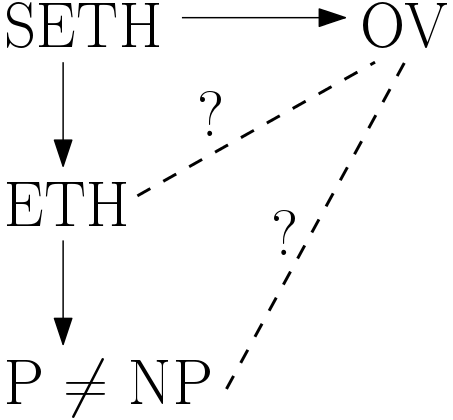
\includegraphics[scale=0.6]{sethOVDiag.png}
%	\caption{The relationships between SETH (strong exponential time hypothesis), ETH (exponential time hypothesis), OV (orthogonal vectors) and P vs NP. The dotted lines signify that we don't know the relationship}
%	\label{fig:sethOVRelationship}
%\end{figure}


%\subsection{Previous Works}
%There has been much prior work leading up to our results. First, there are a few results using assumptions from fine-grained complexity and applying them to cryptography. Second, there has been work with the kind of assumptions that we will be using. 
%
%%TODO: The organization of this section needs work...
%%TODO: merkle puzzles first as weak crypto?
%%TODO: talk about Ball et al stuff first as they try to answer this question, then Vinod's paper, Subset Sum -> k-Sum etc (similar assumptions), and SS -> PKC
%
%
%\subsubsection{Fine-Grained Cryptography}
%Ball et al. \cite{avgCaseFineGrained,eprintAvgCaseFG} considered the key hard problems from fine-grained complexity and showed that one can obtain problems that are hard on average, in a fine-grained sense, using fine-grained worst case to average case reductions. They established useful definitions of fine-grained one-way functions, and derived the first proof-of-work in the fine-grained setting, based on a {\em worst-case} assumption from fine-grained complexity. However, their approach was not sufficient to give a construction of one-way-functions (or public-key cryptography), and indeed Ball et al. proved a limitation of their approach in this regard - extending their approach would falsify the Nondeterministic Strong Exponential Time Hypothesis of Carmosino et al. \cite{CarmosinoGIMPS16}. Because of this seeming barrier, one would either need to develop brand new techniques, or use a different hardness assumption.
%
%
%%These notions are similar to ours in that they make stronger assumptions on the power of an adversary, but while they rely on circuit complexity, which allows them to make unconditional statements, we rely on the more general computational complexity of problems.
%
%
%\paragraph{Fine-Grained Key Exchanges.} Fine-grained cryptography is a relatively unexplored area, even though it had its start in the 1970's with Merkle puzzles: the gap between honestly participating in the protocol versus breaking the security guarantee was only quadratic \cite{Merkle78}. Merkle originally did not describe a plausible hardness assumption under which the security of the key exchange can be based. 30 years later, Biham, Goren, and Ishai showed how to implement Merkle puzzles by making an assumption of the existence of either a random oracle or an exponential gap one way function \cite{BGI08}. That is, Merkle puzzles were built under the assumption that a one-way function exists which takes time $2^{n(1/2+\delta)}$ to invert for some $\delta>0$. So while prior work indeed succeeded in building a fine-grained key-exchange, it need for a very strong variant of OWFs to exist. It is thus very interesting in particular to obtained fine-grained public key encryption schemes based on a fine-grained assumption (and hence might even work in Pessiland and below).
%
%\paragraph{Another notion of Fine-Grained Cryptography.} In 2016, work by Degwekar, Vaikuntanathan, and Vasudevan \cite{DVV16} discussed fine-grained complexity with respect to both honest parties and adversaries restricted to certain circuit classes. They obtained constructions for some cryptographic primitives (including PKE) when restricting an adversary to a certain circuit class. From the assumption $\mathsf{NC}1 \neq \xor L/\poly$ they show Alice and Bob can be in $AC^0[2]$ while being secure against $\mathsf{NC}1$ adversaries. While \cite{DVV16} has some unconditional constructions, their security relies on the circuit complexity of the adversary, and does not apply to arbitrary time-bounded adversaries as is usually the case in cryptography. That is, this restricts the types of algorithms an adversary is allowed to use beyond just how much runtime these algorithms can have. It would be interesting to get similar results in the low-polynomial time regime, without circuit complexity assumptions.
%
%
%
%\begin{figure}
	%\begin{center}
		%\begin{tabular}{| l | l | l | l | l |}
			%\hline
			%Paper & Assumptions & Crypto & Runtime & \begin{tabular}{l} Power of\\ Adversary
			%\end{tabular} \\\hline
			%\cite{Merkle78} & Random Oracles* & Key Exchange & $O(N)$ & $O(N^2)$\\\hline
			%\cite{BGI08} & Exponentially-Strong OWFs & Key Exchange & $O(N)$ & $O(N^2)$ \\\hline
			%\cite{eprintAvgCaseFG} & WC 3-sum, OV, APSP, or SETH & Proof of Work & $O(N^2)$ & N/A \\\hline
			%[This work] & \zkclique~or $k$-sum & \begin{tabular}{l} OWFs,\\
				%Key Exchange \& PKE
			%\end{tabular} &\begin{tabular}{l}
			%$O(N)$\\
			%$O(N)$
		%\end{tabular} & \begin{tabular}{l}
		%$O(N^{1 + \delta})$\\
		%$O(N^{1.5 - \delta})$
	%\end{tabular} \\\hline
	%\cite{DVV16} & $\mathsf{NC}1 \neq \xor L/\poly$ & \begin{tabular}{l}
		%OWFs, and PRGs\\
		%with sublinear \\
		%stretch, CRHFs, \\
		%and PKE\\ \\
	%\end{tabular} &$\mathsf{NC}1$ &$\mathsf{NC}1$\\
	%&$\mathsf{NC}1 \neq \xor L/\poly$ &\begin{tabular}{l} PKE and CRHFs\\ \\
	%\end{tabular}  & $\mathsf{AC}^0[2]$&$\mathsf{NC}1$ \\
	%& Unconditional &\begin{tabular}{l}
		%PRGs with poly\\
		%stretch, Symmetric\\
		%encryption,\\
		%and CRHFs\\
	%\end{tabular}  & $\mathsf{AC}^{0}$ & $\mathsf{AC}^0$\\\hline
%\end{tabular}
%\caption{\label{fig:comparison} A table of previous works' results in this area. There have been several results characterizing different aspects of fine-grained cryptography. *It was \cite{BGI08} who showed that Merkle's construction could be realized with a random oracle. However, Merkle presented the construction.  }
%\end{center}
%\end{figure}
%
%
%
%\subsubsection{Similar Assumptions}
%This paper uses many assumptions that, while solvable in polynomial time, are variants of natural NP-hard problems, in which the size of the solution is a fixed constant. For instance, for constant $k$, $k$-SUM is the variant of Subset Sum, where we are given $n$ numbers and we need to find exactly $k$ elements that sum to a given target, and Zero-$k$-Clique is the variant of Zero-Clique, in which we are given a graph and we need to find exactly  $k$ nodes that form a clique whose edge weights sum to zero.
%
%With respect to Subset Sum, Impagliazzo and Naor showed how to directly obtain OWFs and PRGs assuming that Subset Sum is hard on average \cite{IN02}. The OWF is $f(\vec a, \vec s) = \vec a \cdot \vec s$, where $\vec a$ is the list of elements (chosen uniformly at random from the range $R$) and $s \in \{0,1\}^n$ represents the set of elements we add together.
%In addition to Subset Sum, OWFs have also been constructed from planted Clique, SAT, and Learning-Parity with Noise \cite{Lindell,JP00}. The constructions from \cite{Lindell} come from a definition of a ``plantable'' NP-hard problem that is assumed to be hard on average.
%
%%Although our OWFs are essentially equivalent to scaled-down, polynomial-time solveable characterizations of these problems, we also formalize the property that allows us to get these fine-grained OWFs (plantability). We combine these NP constructions and formalizations to lay the groundwork for fine-grained cryptography.
%
%In more recent work, Subset Sum was also shown to directly imply public-key cryptography \cite{LPS10}. The construction takes ideas from Regev's LWE construction, turning a vector of subset sum elements into a matrix by writing each element out base $q$ in a column. The subset is still represented by a 0-1 matrix, and error is handled by the lack of carrying digits. It is not clear how to directly translate this construction into the fine-grained world, and even less clear what the benefit would be; directly converting from Subset Sum to $k$-Sum just significantly weakens the security without added benefit. A very desirable goal is to obtain novel cryptographic approaches exploiting the fine-grained nature of these problems, going beyond just recasting normal cryptography in the fine-grained world.
%
%

%%%%%%%%%%%%%%%%%%%new work%%%%%%%%%%%%%

\subsection{Our contributions}
%***NEEDS to CHANGE***
%Our main result is a weak key-exchange from a merely polynomial time fine-grained assumption, exploring cryptographic protocols that may maintain security even if $P=NP$. We also obtain a fine-grained version of hardcore bits.

Our main result is a fine-grained key-exchange that can be formed from any problem that meets three structural conditions in the word-RAM model of computation. This addresses the question of what properties are sufficient to produce fine-grained Public Key Encryption schemes (PKEs).
%We show that three properties we define are sufficient to build a fine-grained PKE.


%We describe the assumptions we use and then describe our public key exchange. 
%Then, we explore fine-grained OWFs, showing that hardcore bits, and other basic functionality are not immediate in the fine-grained cryptography world, and also providing a notion of fine-grained hardcore bits that we can achieve. 

For our key exchange, we describe a set of properties, and any problem that has those properties implies a polynomial gap PKE. An informal statement of our main theorem is as follows.\\


\begin{theoremNon}[Fine-Grained Key-Exchange (informal)]
Let $P$ be a computational problem for which a random instance can be generated in $O(n^g)$ time for some $g$, and that
requires $n^{k-o(1)}$ time to be solved on average for some fixed $k>g$.
Additionally, let $P$ have three key structural properties of interest: (1) ``plantable'': we can generate a random-looking instance, choosing either to have or not to have a solution in the instance, and if there is a solution, we know what/where it is; (2)
``average-case list-hard'':  
given a list of $n$ random instances
of the problem, returning which one of the instances has a solution requires essentially
solving all instances;
(3) ``splittable'': when given an instance with a solution, we can
split it in $O(n^g)$ time into two slightly smaller instances that both have solutions.

Then a public key-exchange can be built such that Alice and Bob exchange a $\lg(n)$ bit key in time $n^{2k-g}$, where as Eve must take $\tilde{\Omega}(n^{3k-2g})$ time to learn Alice and Bob's key.
\end{theoremNon}\\

Notice that as long as there is a gap between the time to generate a random instance and the time to solve an instance on average, there is a gap between $N=n^{2k-g}$ and $n^{3k-2g}=N^{3/2 - 1/(4(k/g)-2)}$ and the latter goes to $N^{3/2}$, as $k/g$ grows.
The key exchange requires no interaction, and we get a \emph{fine-grained} public key cryptosystem.
While our key exchange construction provides a relatively small gap between the adversary and the honest parties ($O(N^{1.5})$ vs $O(N)$),  the techniques required to prove security of this scheme are novel and the result is generic as long as the three assumptions are satisfied. In fact, we will show an alternate method to achieve a gap approaching $O(N^2)$ in the full version of this paper.


Our main result above is stated formally and in more generality in Theorem \ref{thm:fg-pkc}. We will explain the formal meaning of our structural properties  \emph{plantable}, \emph{average-case list-hard}, and \emph{splittable} later. 

%(3k-2g)/(2k-g) = *3/2*(2k-g) -0.5g)

We also investigate what plausible average-case assumptions one might be able to make about the key problems from fine-grained complexity so that the three properties from our theorem would be satisfied.
We consider the \zkclique~problem as it is one of the hardest worst-case problems in fine-grained complexity. For instance, it is known that if \zThclique~is in $O(n^{3-\eps})$ time for some $\eps>0$, then both the \ThSum~and the APSP hypotheses are violated \cite{icm-survey,WilliamsW13j}. It is important to note that while fine-grained problems like \zkclique~and \kSum~are suspected to take a certain amount of time in the worst case, when making these assumptions for any constant $k$ does not seem to imply $P \neq NP$ since all of these problems are still solveable in polynomial time.\footnote{Assuming the hardness of these problems for more general $k$ will imply $P \neq NP$, but that is not the focus of our work.}

An instance of \zkclique~is a complete $k$-partite graph $G$, where each edge is given a weight in the range $[0,R-1]$ for some integer $R$. The problem asks whether there is a $k$-clique in $G$ whose edge weights sum to $0$, modulo $R$. A standard fine-grained assumption (see e.g. \cite{icm-survey}) is that in the worst case, for large enough $R$, say $R\geq 10n^{4k}$, \zkclique~requires $n^{k-o(1)}$ time to solve. 
\zkclique~has no non-trivial average-case algorithms for natural distributions (uniform for a range of parameters, similar to \kSum~and Subset Sum). Thus, \zkclique~is a natural candidate for an average-case fine-grained hard problem.
\\

%\begin{theoremNon}[Fine-Grained Key-Exchange (intuitive)]
%	If the zero-$k$-Clique problem is $n^{k-o(1)}$ hard on average then a public key-exchange can be built such that Alice and Bob exchange a $\lg(n)$ bit key in time $n^{2k-2}$, whereas Eve must take $\tilde{\Omega}(n^{3k-4})$ time to learn Alice and Bob's key. 
%\end{theoremNon}
%\\



%Our contribution to this line of work is the first fine-grained key exchange based on a fine-grained combinatorial assumption (see Section \ref{sec:averageCaseAssumptions} for details on our assumption). 

%Because our construction provides a non-interactive key exchange, we also build a public-key cryptosystem out of assumptions that are both combinatorial and related to the assumptions used for one-way functions, as opposed to those used for trap-door functions.

Our other contribution addresses an open question from Ball et al.: can a fine-grained one-way function be constructed from worst case assumptions? While we do not fully achieve this, we generate new plausible average-case assumptions from fine-grained problems that imply fine-grained one-way functions. %We also explore how these fine-grained OWFs can generate fine-grained hardcore bits. The standard Goldreich-Levin construction \cite{hardCoreBitsAndXorLemmaFromGL} does not directly work, so we devise a natural variant of fine-grained hardcore bits and develop methods to generate them.


\subsection{Previous Works}
There has been much prior work leading up to our results. First, there are a few results using assumptions from fine-grained complexity and applying them to cryptography. Second, there has been work with the kind of assumptions that we will be using. 

%TODO: The organization of this section needs work...
%TODO: merkle puzzles first as weak crypto?
%TODO: talk about Ball et al stuff first as they try to answer this question, then Vinod's paper, Subset Sum -> k-Sum etc (similar assumptions), and SS -> PKC


\subsubsection{Fine-Grained Cryptography}
Ball et al. \cite{avgCaseFineGrained,eprintAvgCaseFG} produce fine-grained wost-case to average-case reductions. Ball et al. leave an open problem of producing a one-way-function from a worst case assumption. They prove that from some fine-grained assumptions building a one-way-function would falsify NSETH \cite{CarmosinoGIMPS16}\cite{avgCaseFineGrained}.
%Ball et al. \cite{avgCaseFineGrained,eprintAvgCaseFG} considered the key hard problems from fine-grained complexity and showed that one can obtain problems that are hard on average, in a fine-grained sense, using fine-grained worst-case to average-case reductions. They established useful definitions of fine-grained one-way functions, and derived the first proof-of-work in the fine-grained setting, based on a {\em worst-case} assumption from fine-grained complexity. However, their approach was not sufficient to give a construction of one-way-functions (or public-key cryptography), and indeed Ball et al. proved a limitation of their approach in this regard - extending their approach would falsify the Nondeterministic Strong Exponential Time Hypothesis of Carmosino et al. \cite{CarmosinoGIMPS16}. Because of this seeming barrier, one would either need to develop brand new techniques, or use a different hardness assumption.
We avoid their barrier in this paper by producing a construction of both fine-grained OWFs and fine-grained PKE from an \emph{average-case} assumption.
%We choose to do the latter in this paper, producing a construction of both fine-grained OWFs and fine-grained PKE from an \emph{average-case} assumption. So, the question of how to build OWFs from worst case fine-grained complexity assumptions that was left open by Ball et al. is still open. However, our demonstration of explicit constructions for a fine-grained PKE from polynomial problems begins to classify what polynomial time assumptions result in public key cryptography. %opens the possibility of cryptography when no strong OWFs exist. 


%However, Merkel puzzle constructions require a OWF that is not invertible in $2^{n(\frac{1}{2}+\epsilon)}$ time for some $\epsilon>0$. So while this is a fine-grained exponential assumption, we only require a fine-grained polynomial assumption.




\paragraph{Fine-Grained Key Exchanges.} Fine-grained cryptography is a relatively unexplored area, even though it had its start in the 1970's with Merkle puzzles: the gap between honestly participating in the protocol versus breaking the security guarantee was only quadratic \cite{Merkle78}. Merkle originally did not describe a plausible hardness assumption under which the security of the key exchange can be based. 30 years later, Biham, Goren, and Ishai showed how to implement Merkle puzzles by making an assumption of the existence of either a random oracle or an exponential gap one way function \cite{BGI08}. That is, Merkle puzzles were built under the assumption that a one-way function exists which takes time $2^{n(1/2+\delta)}$ to invert for some $\delta>0$. So while prior work indeed succeeded in building a fine-grained key-exchange, it needed a very strong variant of OWFs to exist. It is thus very interesting to obtain fine-grained public key encryption schemes based on a fine-grained assumption (that might even work in Pessiland and below).

%Considering Merkle Puzzles and other cryptographic assumptions, one may be concerned that a fine-grained assumption is as strong as, say, assuming that exponentially-hard OWFs exist. However, these two assumptions are essentially orthogonal to each other, and in some senses standard cryptographic assumptions are stronger. For example, the standard notion of OWFs trivially imply that fine-grained OWFs exist, but there is no known way of showing the reverse.

% Merkel Puzzles
%The known constructions of Merkle puzzles produce fine-grained PKE from fine-grained exponential OWFs \cite{Merkle78,BGI08,optimalMerklePuzzles}. We are able to build a only slightly weaker PKE from a \textit{polynomial} time hardness assumption. Furthermore, we show that a class of  polynomial time fine-grained assumptions lead to fine-grained PKEs.%As we mentioned earlier, our assumption might still hold even if exponential OWFs do not exist.
%TODO: make sure this meshes with the above

\paragraph{Another notion of Fine-Grained Cryptography.} In 2016, work by Degwekar, Vaikuntanathan, and Vasudevan \cite{DVV16} discussed fine-grained complexity with respect to both honest parties and adversaries restricted to certain circuit classes. They obtained constructions for some cryptographic primitives (including PKE) when restricting an adversary to a certain circuit class. From the assumption $\mathsf{NC}1 \neq \xor L/\poly$ they show Alice and Bob can be in $AC^0[2]$ while being secure against $\mathsf{NC}1$ adversaries. While \cite{DVV16} obtains some unconditional constructions, their security relies on the circuit complexity of the adversary, and does not apply to arbitrary time-bounded adversaries as is usually the case in cryptography. That is, this restricts the types of algorithms an adversary is allowed to use beyond just how much runtime these algorithms can have. It would be interesting to get similar results in the low-polynomial time regime, without restricting an adversary to a certain circuit class. Our results achieve this, though not unconditionally.

\paragraph{Tight Security Reductions and Fine-Grained Crypto.}
Another area the world of fine-grained cryptography collides with is that of tight security reductions in cryptography. Bellare et.al. coined the term ``concrete'' security reductions in \cite{BellareKR94,BellareGR95}. Concrete security reductions are parametrized by time ($t$), queries ($q$), size ($s$), and success probability ($\eps$). 
%This definition stated that a program (adversary) could only run in time $t$, making $q$ queries of size at most $\ell$, to some oracle for a function, can only succeed with probability at most $\epsilon$ in solving some problem.
This line of work tracks how a reduction from a problem to a  construction of some cryptographic primitive effects the four parameters of interest.  
%This line of work relies on seeing how exactly a reduction from a problem that is $(t,q,\ell,\epsilon)$-secure to a construction of some cryptographic primitive is comparably secure, keeping track of how $t$, $q$, $\ell$, and $\epsilon$ change. 
This started a rich field of study connecting theory to practical cryptographic primitives (such as PRFs, different instantiations of symmetric encryption, and even IBE for example \cite{BellareCK96,BellareDJR97,KatzW03,BellareR09}). %Since we are not guaranteed much in terms of security or even a negligible advantage in our fine-grained setting, 
In fine-grained reductions we also need to track exactly how our adversary's advantage changes throughout our reductions, however, we also track the running time of the honest parties. % --- at least up to the nearest polynomial. However, we also seek to convey the security in our constructions in a way that makes it relatively easy to compose schemes without needing to worry too much about runtime. 
So, unlike in the concrete security literature, when the hard problems are polynomially hard (perhaps because $P=NP$), we can track the gap in running times between the honest and dishonest parties. This allows us to build one way functions and public key cryptosystems when the hard problems we are given are only polynomially hard. 
%So, unlike in the concrete security literature, we ignore log factors and instead focus on $\~O$ notation.
%%%TODO: this is not a convincing differece between their work and ours

\vspace{-0.5cm}

\begin{figure}
	\begin{center}
		\begin{tabular}{| l | l | l | l | l |}
			\hline
			Paper & Assumptions & Crypto & Runtime & \begin{tabular}{l} Power of\\ Adversary
			\end{tabular} \\\hline
			\cite{Merkle78} & Random Oracles* & Key Exchange & $O(N)$ & $O(N^2)$\\\hline
			\cite{BGI08} & Exponentially-Strong OWFs & Key Exchange & $O(N)$ & $O(N^2)$ \\\hline
			\cite{eprintAvgCaseFG} & WC \ThSum, OV, APSP, or SETH & Proof of Work & $O(N^2)$ & N/A \\\hline
			[This work] & \zkclique~or \kSum& \begin{tabular}{l} OWFs,\\
				Key Exch. \& PKE
			\end{tabular} &\begin{tabular}{l}
			$O(N)$\\
			$O(N)$
		\end{tabular} & \begin{tabular}{l}
		$O(N^{1 + \delta})$\\
		$O(N^{1.5 - \delta})$
	\end{tabular} \\\hline
	\cite{DVV16} & $\mathsf{NC}1 \neq \xor L/\poly$ & \begin{tabular}{l}
		OWFs, and PRGs\\
		with sublinear \\
		stretch, CRHFs, \\
		and PKE\\ \\
	\end{tabular} &$\mathsf{NC}1$ &$\mathsf{NC}1$\\
	&$\mathsf{NC}1 \neq \xor L/\poly$ &\begin{tabular}{l} PKE and CRHFs\\ \\
	\end{tabular}  & $\mathsf{AC}^0[2]$&$\mathsf{NC}1$ \\
	& Unconditional &\begin{tabular}{l}
		PRGs with poly\\
		stretch, Symmetric\\
		encryption,\\
		and CRHFs\\
	\end{tabular}  & $\mathsf{AC}^{0}$ & $\mathsf{AC}^0$\\\hline
\end{tabular}
\caption{\label{fig:comparison} A table of previous works' results in this area. There have been several results characterizing different aspects of fine-grained cryptography. *It was \cite{BGI08} who showed that Merkle's construction could be realized with a random oracle. However, Merkle presented the construction.  }
\end{center}
\end{figure}
%\vspace{-1.22cm}
\subsubsection{Similar Assumptions}
This paper uses hypotheses on the running times of problems that, while solvable in polynomial time, are variants of natural NP-hard problems, in which the size of the solution is a fixed constant. For instance, \kSum~is the variant of Subset Sum, where we are given $n$ numbers and we need to find exactly $k$ elements that sum to a given target, and \zkclique~is the variant of Zero-Clique, in which we are given a graph and we need to find exactly $k$ nodes that form a clique whose edge weights sum to zero.

With respect to Subset Sum, Impagliazzo and Naor showed how to directly obtain OWFs and PRGs assuming that Subset Sum is hard on average \cite{IN02}. The OWF is $f(\vec a, \vec s) = (\vec a, \vec a \cdot \vec s)$, where $\vec a$ is the list of elements (chosen uniformly at random from the range $R$) and $s \in \{0,1\}^n$ represents the set of elements we add together.
In addition to Subset Sum, OWFs have also been constructed from planted Clique, SAT, and Learning-Parity with Noise \cite{Lindell,JP00}. The constructions from the book of Lindell and the chapter written by Barak \cite{Lindell} come from a definition of a ``plantable'' NP-hard problem that is assumed to be hard on average.

Although our OWFs are equivalent to scaled-down, polynomial-time solvable characterizations of these problems, we also formalize the property that allows us to get these fine-grained OWFs (plantability). We combine these NP constructions and formalizations to lay the groundwork for fine-grained cryptography.

In the public-key setting, there has been relatively recent work taking NP-hard problems and directly constructing public-key cryptosystems \cite{ABW10}. They take a problem that is NP-hard in its worst case and come up with an average-case assumption that works well for their constructions. Our approach is similar, and we also provide evidence for why our assumptions are correct.

In recent work, Subset Sum was also shown to directly imply public-key cryptography \cite{LPS10}. The construction takes ideas from Regev's LWE construction \cite{Regev05}, turning a vector of subset sum elements into a matrix by writing each element out base $q$ in a column. The subset is still represented by a 0-1 matrix, and error is handled by the lack of carrying digits. It is not clear how to directly translate this construction into the fine-grained world. First, directly converting from Subset Sum to \kSum~just significantly weakens the security without added benefit. More importantly, the security reduction has significant polynomial overhead, and would not apply in a very pessimistic Pessiland where random planted Subset Sum instances can be solved in quadratic time, say.

While it would be interesting to reanalyze the time-complexity of this construction (and others) in a fine-grained way, this is not the focus of our work. Our goal is to obtain novel cryptographic approaches exploiting the fine-grained nature of the problems, going beyond just recasting normal cryptography in the fine-grained world, and obtaining somewhat generic constructions.


\subsection{Technical Overview}
Here we will go into a bit more technical detail in describing our results. First, we need to describe our hardness assumptions. Then, we will show how to use them for our fine-grained key exchange, and finally, we will talk briefly about fine-grained OWFs and hardcore bits.

\paragraph{Our Hardness Assumption} %TODO: Be precise about modulus etc

We generate a series of properties where if a problem has these properties then a fine-grained public key-exchange can be built.

One property we require is that the problem is hard on average, in a fine-grained sense. Intuitively, a problem is average case indistinguishably hard if given an instance that is drawn with probability $1/2$ from instances with no solutions and with probability $1/2$ from instances with one solution, it is computationally hard on average to distinguish whether the instance has $0$ or $1$ solutions.
The rest of the properties are structural; we need a problem that is \emph{plantable}, \emph{average-case list-hard}, and \emph{splittable}. Informally,

\begin{itemize}
	\item The plantable property roughly says that one can efficiently choose to generate either an instance without a solution or one with a solution, knowing where the solution is; %A problem is plantable if, we can generate a random-looking instance, choosing either to have or not to have a solution in the instance, and if there is a solution, we know what/where it is;
	%when given a random instance without a solution, we can \emph{plant} one, and have the resulting output ``look'' random;
	\item The average case list-hard property says that if one is given a list of instances where all but one of them are drawn uniformly over instances with no solutions, and a random one of them is actually drawn uniformly from instances with one solution, then it is computationally hard to find the instance with a solution;
	\item Finally, the splittable property says that one can generate from one average case instance, two new average case instances that have the same number of solutions as the original one. %A problem is splittable if when given an instance with a solution, we can split it into two slightly smaller instances that \emph{both} have solutions.
\end{itemize}
These are natural properties for problems and hypotheses to have. We will demonstrate in Section \ref{sec:zkcIsAllTheThings} that \zkclique~has all of these properties. We need our problem to have all three of these qualities for the key exchange. For our one-way function constructions we only need the problem to be plantable.

%The strong version of our \zkclique~assumption satisfies all of three of these properties. %For the remainder of this overview, we will be using the assumption that we can generate a planted \zkclique~instance in time $O(n^2)$ and it takes $O(n^k)$ for any randomized adversary to find the clique. In section \ref{sec:fg-owfs}, we show that we can relax this assumption for constructing both key exchanges and fine-grained OWFs.

%Usefully, our properties also immediately imply the existence of a fine-grained one-way function based on the problem that satisfies them.

The structural properties are quite generic, and in principle, there could be many problems that satisfy them. We exhibit one: the \zkclique~problem.

Because no known algorithmic techniques seem to solve \zkclique~even when the weights are selected independently uniformly at random from $[0,cn^k]$ for a constant $c$, folklore intuition dictates that the problem might be hard on average for this distribution: here, the expected number of $k$-Cliques is $\Theta(1)$, and solving the decision problem correctly on a large enough fraction of the random instances seems difficult.
This intuition was formally proposed by Pettie~\cite{avgCase3Sum} for the very related \kSum~problem which we also consider.

We show that the \zkclique~problem, together with the assumption that it is fine-grained hard to solve on average, satisfies all of our structural properties, and thus, using our main theorem, one can obtain a fine-grained key exchange based on 
\zkclique.

\textit{Key Exchange Assumption.} We assume that when given a complete $k$-partite graph with $kn$ nodes and random weights $[0,R-1]$, $R = \Omega(n^k)$, any adversary running in time $n^{k-\Omega(1)}$ time cannot distinguish an instance with a zero-$k$-clique solution from one without with more than $2/3$ chance of success.
In more detail, consider a distribution where with probability $1/2$ one generates a random instance of size $n$ with no solutions, and with probability $1/2$ one generates a random instance of size $n$ with exactly one solution. (We later tie in this distribution to our original uniform distribution.) Then, consider an algorithm that can determine with probability $2/3$ (over the distribution of instances) whether the problem has a solution or not.
%We first hypothesize that any such algorithm for \kSum~or \zkclique~must take super-linear time. From this weak assumption we can get one-way functions. 
We make the conjecture that such a $2/3$-probability distinguishing algorithm for \zkclique, which can also exhibit the unique zero clique whenever a solution exists, 
requires time $n^{k-o(1)}$.



\paragraph{Public Key Exchange}

So, what does the existence of a problem with our three properties, \emph{plantable}, \emph{average-case list-hard}, and \emph{splittable}, imply?

The intuitive statement of our main theorem is that, if a problem has the three properties, and is $n^k$ hard to solve on average and can be generated in $n^g$ time (for \zkclique~$g=2$), then a key exchange exists that takes $O(N)$ time for Alice and Bob to execute, and requires an eavesdropper Eve $\tilde{\Omega}(N^{(3k-2g)/(2k-g)})$ time to break. When $k>g$ Eve takes super linear time in terms of $N$. When $k=3$ and $g=2$, an important case for the \zkclique~problem, Eve requires $\tilde{\Omega}(N^{5/4})$ time. 

For the rest of this overview we will describe our construction with the problem \zkclique. 

To describe how we get our key exchange, it is first helpful to consider Merkle Puzzles \cite{Merkle78,BGI08,optimalMerklePuzzles}. The idea is simple: let $f$ be a one way permutation over $n$ bits (so a range of $2^n$ values) requires $2^{n(\frac{1}{2}+\epsilon)}$ time to invert for some constant $\epsilon>0$. Then, Alice and Bob could exchange a key by each computing $f(v)$ on  $10\cdot2^{n/2}$ random element $v \in [2^{n}]$ and sending those values $f(v)$ to each other. With .9 probability, Alice and Bob would agree on at least one pre-image, $v$. It would take an eavesdropper Eve $\Omega(2^{n(\frac{1}{2}+\epsilon)})$ time before she would be able to find the $v$ agreed upon by Alice and Bob. So, while Alice and Bob must take $O(2^{n/2})$ time, Eve must take $O(2^{n(\frac{1}{2}+\epsilon)})$ time to break it. 

%Specifically, assume there exists a one way function, $f$, over $\{0,1\}^n$ that can be computed in polynomial time, but requires $2^{n(\frac{1}{2}+\epsilon)}$ time to invert. Then, using Merkle Puzzles, the two honest parties, Alice and Bob could do $N=\Theta^*(2^{n/2})$ work to exchange an index of size $\lg(N)=n$. If an eavesdropper Eve wanted to also learn the key, she would need to put in $N^{1+2\epsilon}=\Omega^*(2^{n(\frac{1}{2}+\epsilon)})$ work. 

%\emph{fine-grained} exponential assumption. The assumption is simultaneously exponential and sensitive to multiplicative constants. Notably, a one way permutation that requires $2^{n\frac{1}{3}}$ time to invert does not imply the existence of a fine-grained key-exchange via this strategy. 

Our construction will take on a similar form: Alice and Bob will send several problems to each other, and some of them will have planted solutions. By matching up where they both put solutions, they get a key exchange.

Concretely, Alice and Bob will exchange $m$ instances of the \zkclique~problem and in $\sqrt{m}$ of them (chosen at random), plant solutions. The other $m - \sqrt{m}$ will not have solutions (except with some small probability). These $m$ problems will be indexed, and we expect Alice and Bob to have both planted a solution in the same index. Alice can check her $\sqrt{m}$ indices against Bob's, while Bob checks his, and by the end, with constant probability, they will agree on a single index as a key. In the end, Alice and Bob require $O(mn^g + \sqrt{m}n^{k})$ time to exchange this index.  Eve must take time $\tilde{\Omega}(n^{k}m)$. When  $m = n^{2k-2g}$, Alice and Bob take $O(n^{2k-g})$ time and Eve takes $\tilde{\Omega}(n^{3k-2g})$. We therefore get some gap between the running time of Alice and Bob as compared to Eve for any value of $k\geq g$. Furthermore, for all $\delta>0$ there exists some large enough $k$ such that the difference in running time is at least $O(T(n))$ time for Alice and Bob and $\tilde{\Omega}(T(n)^{1.5-\delta})$ time for Eve. Theorem \ref{thm:fg-pkc} is the formal theorem statement.



\begin{figure}[h]
	\centering
	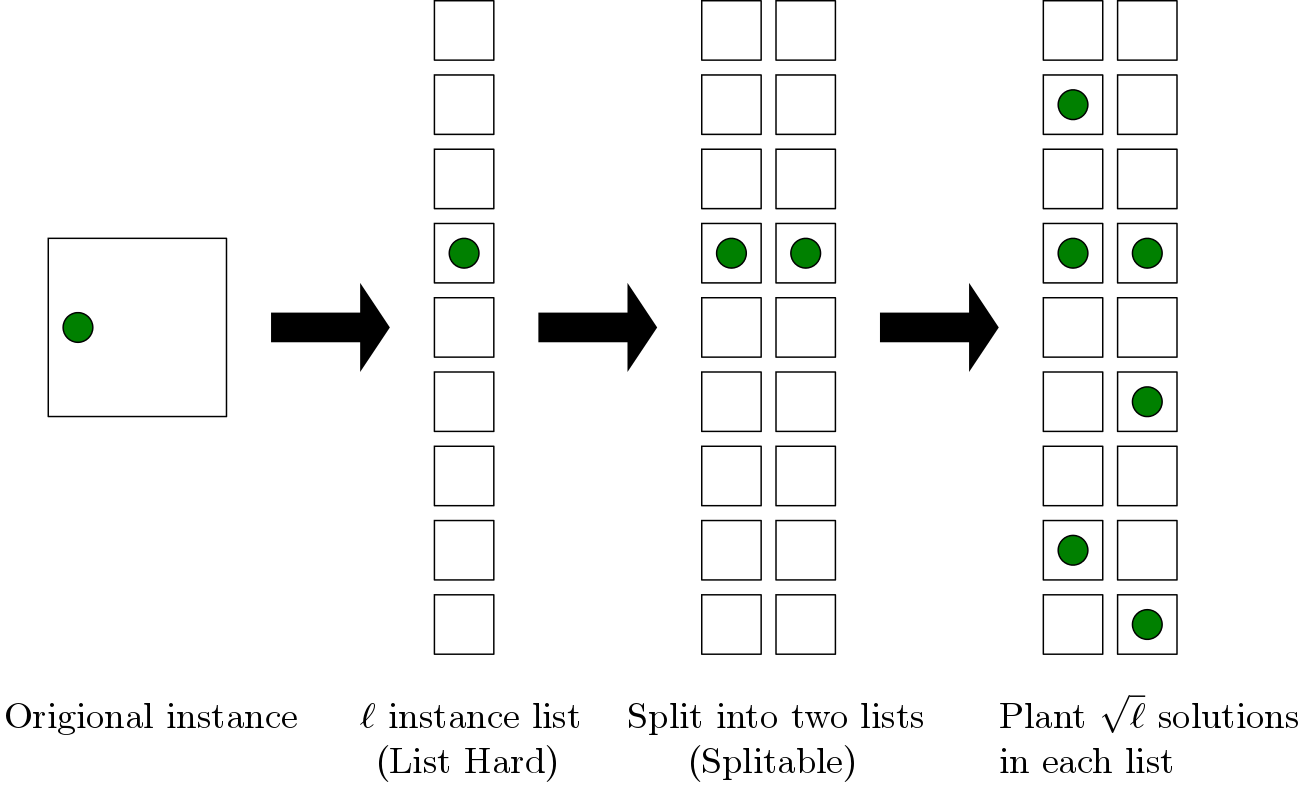
\includegraphics[scale=0.6]{fgcrypto/FullReduction.png}
	\caption{A depiction of our reduction showing hardness for our fine-grained key exchange.}
	\label{fig:wholeReductionBoxes}
\end{figure}

To show hardness for this construction we combine techniques from both fine-grained complexity and cryptography (see Figure \ref{fig:wholeReductionBoxes}). We take a single instance and use a self-reduction to produce a list of $\ell$ instances where one has a solution whp if the original instance has a solution. In our reductions $\ell$ will be polynomial in the input size. Then, we take this list and produce two lists that have a solution in the same location with high probability if the original instance has a solution. Finally, we plant $\sqrt{\ell}$ solutions into the list, to simulate Alice and Bob's random solution planting. 

%\xxx{Rio: Need to put a theorem statement in here}
%\begin{theorem}[Fine-Grained Key-Exchange (informal)]
%Let $P$ be an average case problem that can be generated and planted in time $n^2$, but requires $n^{k-o(1)}$ to be solved where $k>2$. Additionally, let $P$ be \emph{plantable}, \emph{average-case list-hard}, and \emph{splittable}.

%Then a public key-exchange can be built such that Alice and Bob exchange a $\lg(n)$ bit key in time $n^{2k-2}$, where as Eve must take $\tilde{\Omega}(n^{3k-4})$ time to learn Alice and Bob's key. 
%\end{theorem}


%We present a set of three general properties where if a problem has those properties then a fine-grained key exchange exists. These properties are that the problem must be \emph{plantable}, \emph{average }


\paragraph{One Way Functions}
%\xxx{Rio: Need to rewrite to put in context of other OWF definitions. Also note the Yao part.}
First, and informally, a fine-grained OWF is a function on $n$ bits that requires $\~O(T(n)^{1-\delta})$ time to evaluate for some constant $\delta > 0$, and if any adversary attempts to invert $f$ in time $\~O(T(n)^{1 - \delta'})$ for \emph{any} constant $\delta' > 0$, she only succeeds with probability at most $\epsilon(n)$, where $\epsilon$ is considered ``insignificant.''

Ball et al. \cite{avgCaseFineGrained} defined fine-grained OWFs, keeping track of the time required to invert and the probability of inversion in two separate parameters. We streamline this definition by fixing the probability an adversary inverts too an insignificant function of input size, which we define in Section \ref{sec:prelims}. %It will turn out that this notion of insignificance will extend to our definition of hardcore bits.

For this overview, we will focus on the intuition of using specific problems \kSum-$R$ (\kSum~modulo $R$) or \zkclique-$R$ (\zkclique~modulo $R$) to get fine-grained OWFs, though in section \ref{sec:fg-owfs}, we construct fine-grained OWFs from a general class of problems. Let $N$ be the size of the input to these problems. Note that if $R$ is too small (e.g. constant), then these problems are solvable quickly and the assumptions we are using are false. So, we will assume $R = \Omega(n^k)$.

\textit{OWF Assumptions.} Much like for our key exchange, our assumptions are about the difficulty of distinguishing an instance of \kSum~or \zkclique~with probability more than $2/3$ in time faster than $n^{k/2}$ or $n^k$ respectively. Formally, randomly generating a \kSum-$R$ instance is creating a $k$ lists of size $n$ with values randomly chosen from $[0,R-1]$. Recall that a random \zkclique~instance is a complete $k$-partite graph where weights are randomly chosen from $[0,R-1]$. Our `weak' \kSum-$R$ and \zkclique-$R$ assumptions state that for any algorithm running in $O(n)$ time, it cannot distinguish between a randomly generated instance with a planted solution and one without with probability greater than $2/3$.

Note that these assumptions are much weaker than the previously described key-exchange assumption, where we allowed the adversary $O(n^{k-\Omega(1)})$ time instead of just super-linear.

\begin{theorem}[Fine-Grained OWFs (informal)]
	If for some constant $\delta>0$ and range $R = \Omega(n^k)$ either \kSum-$R$ requires $\Omega(N^{1+\delta})$ time to solve with probability $>2/3$ or \zkclique-$R$ requires $\Omega(N^{(1+\delta)})$ time to solve with probability $>2/3$  then a fine-grained OWF exists.
\end{theorem}
The formal theorem is Theorem \ref{thm:FGOWFs-exist} and is proved in Appendix \ref{sec:building-fgowfs}.

Intuitively our construction of a fine-grained OWF runs a planting procedure on a random instance in time $O(N)$. By our assumptions finding this solution takes time $\Omega(N^{1+\delta})$ for some constant $\delta > 0$, and thus inverting this OWF takes $\Omega(N^{1+\delta})$.

We also get a notion of hardcore bits from this. Unlike in traditional crypto, we can't immediately use Goldreich-Levin's hardcore bit construction \cite{hardCoreBitsAndXorLemmaFromGL}. Given a function on $N$ bits, the construction requires at least $\Omega(N)$ calls to the adversary who claims to invert the hardcore bit. When one is seeking super-polynomial gaps between computation and inversion of a function, factors of $N$ can be ignored. However, in the fine-grained setting, factors of $N$ can completely eliminate the gap between computation and inversion, and so having a notion of fine-grained hardcore bits is interesting.

We show that for our concrete constructions of fine-grained OWFs, there is a subset of the input of size $O(\lg(N))$ (or any sub-polynomial function) which itself requires $\Omega(N^{1+\delta})$ time to invert. From this subset of bits we can use Goldreich-Levin's hardcore bit construction, only losing a factor of $N^{o(1)}$ which is acceptable in the fine-grained setting.

\begin{theorem}[Hardcore Bits (informal)]
	If for some constant $\delta>0$ and range $R = \Omega(n^k)$ either \kSum-$R$ requires $\Omega(N^{1+\delta})$ time to solve with probability $>2/3$ or \zkclique-$R$ requires $\Omega(N^{1+\delta})$ time to solve with probability $>2/3$  then a fine-grained OWF exists with a hardcore bit that can not be guessed with probability greater than $\frac 1 2 +1/q(n)$ for any $q(n) = n^{o(1)}$.
\end{theorem}
The formal theorem is Theorem \ref{thm:fine-grained-GL} and is proved in Appendix \ref{sec:fg-hardcore-bits}.

Intuitively, solutions for \kSum-$R$ and \zkclique-$R$ can be described in $O(\log(n))$ bits --- we just list the locations of the solution. Given a solution for the problem, we can just change one of the weights and use the solution location to produce a correct preimage. So, now using Goldreich-Levin, we only need to make $O(\log(n))$ queries during the security reduction.

%%%%%%%%%%%%%%%%%OLD STUFF%%%%%%%%%%%%%%%%%%%


%Prior approaches needed to assume that a problem is super-polynomially hard to solve (like inverting an exponentially strong one-way function), or that random oracles exist. Our work identifies a handful of structural properties, so that if a computational problem satisfies them, then we can build a fine-grained key exchange from it.


%In addition to our constructions, we explore average-case to average-case reductions between fine-grained problems. In particular, we are able to show a reduction from an instance of average-case \zkclique~to breaking our key exchange. %Interestingly, this reduction fails in the worst case! 
%This motivates further research into getting better average-case reductions for fine-grained problems, and even worst-case to average-case reductions for these problems in general.

%Along that line of reasoning, Ball, Rosen, Sabin, and Vasudevan published a work establishing the definition of fine-grained one-way functions, and importantly got the first worst-case to average-case reduction from one fine-grained problem to another \cite{avgCaseFineGrained}. However, while they were able to make progress in worst-case to average-case reduction, they were unable to construct one-way functions based off of these problems, and even presented barriers for why one would be difficult or impossible to construct.
%



\subsection{Organization of Paper}

In section \ref{sec:prelims} we define our notions of fine-grained crypto primitives, including fine-grained OWFs, fine-grained hardcore bits, and  fine-grained key exchanges. In section \ref{sec:averageCaseAssumptions}, we describe a few classes of general assumptions (plantable, splittable, and average-case list hard), and then describe the concrete fine-grained assumptions we use (\kSum~and \zkclique). Next, in section \ref{sec:justifyAssumptions} we show that the concrete assumptions we made imply certain subsets of the general assumptions. 
%Then, in our next two sections, we describe how to use our general assumptions to get our fine-grained crypto primitives. 
In section \ref{sec:FineGrainedKeyExchange}, we show that using an assumption that is plantable, splittable, and average-case list hard, we can construct a fine-grained key exchange.
%Finally, we conclude with some open problems in this area in section \ref{sec:future work}.

In the supplementary appendix section \ref{sec:fg-owfs}, we show how to use a plantable problem to get a fine-grained OWF.
In supplementary materials section \ref{sec:kcliqueksumAllTHeThings} we show that \zkclique~has all of the desired properties (plantable, splittable, and average-case list hard).
